\section{Introduction}
\begin{figure}[h]
\centering
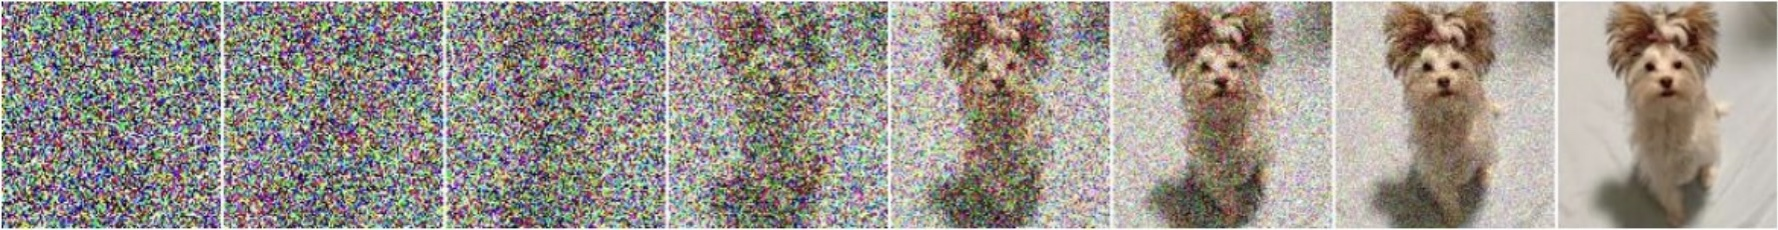
\includegraphics[width=\textwidth]{images/diffusion.png}
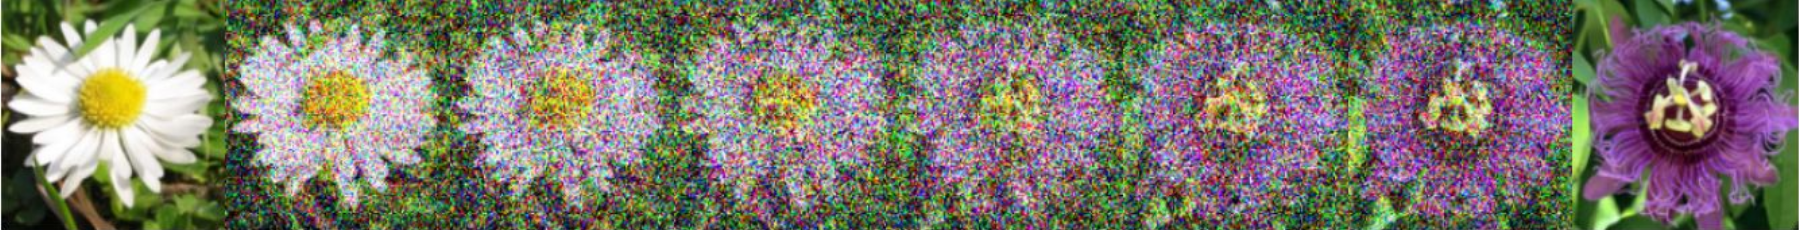
\includegraphics[width=\textwidth]{images/bridge.png}
\caption{Top: denoising process, defined by a diffusion model~\cite{song2020score}. Bottom: stochastic interpolation between two pictures~\cite{albergo2023stochastic}.}
\end{figure}

This tutorial aims to introduce the reader to the mathematical methods which are widely used in contemporary generative modeling. Big practical success of diffusion models~\cite{ho2020denoising, de2021diffusion, song2020score}, which generate a sequence of pictures instead of just the target one, led to development of a novel family of models that describe some dynamic processes. Almost all processes occuring in the real world can be described by differential equations, which will be the basis of the generative models reviewed here. We will cover methods based on either ordinary (ODE) or stochastic (SDE) differential equations, applicable for generation~\cite{song2020score, lipman2022flow, tong2023conditional, albergo2022building, albergo2023stochastic}, paired~\cite{tong2023conditional, albergo2022building, albergo2023stochastic, liu20232} and unpaired~\cite{liu2022flow, shi2023diffusion, korotin2022neural, gushchin2022entropic} domain translation, formalized as an instance of the optimal transport problem.
